\section*{Trigonometrie}
\begin{multicols}{3}

\small
\begin{multicols}{2}
\subsection*{Identitäten}

\textbf{Kofunktionen}
\begin{align*}
    & \sin(\frac{\pi}{2} - x) & = \cos x \\
    & \cos(\frac{\pi}{2} - x) & = \sin x \\
    & \tan(\frac{\pi}{2} - x) & = \cot x \\
    & \cot(\frac{\pi}{2} - x) & = \tan x \\
    & \sec(\frac{\pi}{2} - x) & = \csc x \\
    & \csc(\frac{\pi}{2} - x) & = \sec x
\end{align*}
\textbf{Symmetrie}
\begin{align*}
  \sin(-x) & = - \sin x \\
  \cos(-x) & = \cos x   \\
  \tan(-x) & = -\tan x
\end{align*}
\textbf{Doppelter Winkel}
\begin{align*}
  \sin(2x) & = 2 \sin x \cos x               \\
  \cos(2x) & = \cos^2 x - \sin^2 x           \\
           & = 2 \cos^2 x - 1                \\
           & = 1 - 2 \sin^2 x                \\
  \tan(2x) & = \frac{2 \tan x}{1 - \tan^2 x}
\end{align*}
\textbf{Halber Winkel}
\begin{align*}
  \sin \frac{x}{2} & = \pm \sqrt{ \frac{1 - \cos x }{2} } \\
  \cos \frac{x}{2} & = \pm \sqrt{ \frac{1 + \cos x }{2} } \\
  \tan \frac{x}{2} & = \frac{1 - \cos x }{\sin x}         \\
                   & = \frac{ \sin x }{ 1 + \cos x }
\end{align*}
\textbf{Exponent Reduktion}
\begin{align*}
  \sin^2 x & = \frac{1 - \cos 2x}{2}               \\
  \sin^4x  & = (\frac{1 - \cos 2x}{2})^2           \\
  \cos^2 x & = \frac{1 + \cos 2x}{2}               \\
  \cos^4x  & = (\frac{1 + \cos 2x}{2})^2           \\
  \tan^2 x & = \frac{1 - \cos 2x}{1 + \cos 2x}     \\
  \tan^4 x & =( \frac{1 - \cos 2x}{1 + \cos 2x})^2
\end{align*}
\textbf{Pythagoras}
\begin{align*}
  \sin^2 x + \cos^2 x & = 1        \\
  1 + \tan^2 x        & = \sec^2 x \\
  1 + \cot^2 x        & = \csc^2 x
\end{align*}
\textbf{Umkehrwert}
\begin{align*}
  \cot x & = \frac{1}{\tan x} \\
  \csc x & = \frac{1}{\sin x} \\
  \sec x & = \frac{1}{\cos x}
\end{align*}
\textbf{Quotient}
\begin{align*}
    \tan(x) = \frac{\sin(x)}{\cos(x)}\\
    \cot(x) = \frac{\cos(x)}{\sin(x)}
\end{align*}
\end{multicols}
\textbf{Summe und Differenz von Winkel}
\begin{align*}
  \sin(x + y) & = \sin x \cos y + \cos x \sin y             \\
  \sin(x - y) & = \sin x \cos y - \cos x \sin y             \\
  \cos(x + y) & = \cos x \cos y - \sin x \sin y             \\
  \cos(x - y) & = \cos x \cos y + \sin x \sin y             \\
  \tan(x + y) & = \frac{\tan x + \tan y}{1 - \tan x \tan y} \\
  \tan(x - y) & = \frac{\tan x - \tan y}{1 + \tan x \tan y}
\end{align*}
\textbf{Produkt zu Summe}
\begin{align*}
  \sin x \sin y & = \frac{1}{2}\big[\cos(x - y) - \cos(x + y)\big] \\
  \cos x \cos y & = \frac{1}{2}\big[\cos(x - y) + \cos(x + y)\big] \\
  \sin x \cos y & = \frac{1}{2}\big[\sin(x + y) + \sin(x - y)\big] \\
  \tan x \tan y & = \frac{ \tan x + \tan y }{ \cot x + \cot y }    \\
  \tan x \cot y & = \frac{ \tan x + \cot y }{ \cot x + \tan y }
\end{align*}
\textbf{Summe Zu Produkt}
\begin{align*}
  \sin x + \sin y & = 2 \sin \Big( \frac{x + y}{2} \Big) \cos \Big( \frac{x - y}{2} \Big)  \\
  \sin x - \sin y & = 2 \cos \Big( \frac{x + y}{2} \Big) \sin \Big( \frac{x - y}{2} \Big)  \\
  \cos x + \cos y & = 2 \cos \Big( \frac{x + y}{2} \Big) \cos \Big( \frac{x - y}{2} \Big)  \\
  \cos x - \cos y & = -2 \sin \Big( \frac{x + y}{2} \Big) \sin \Big( \frac{x - y}{2} \Big) \\
  \tan x + \tan y & = \frac{ \sin(x + y) }{ \cos x \cos y}                                 \\
  \tan x - \tan y & = \frac{ \sin(x - y) }{ \cos x \cos y}                                 \\
\end{align*}
\textbf{Additionstheoreme}
\begin{align*}
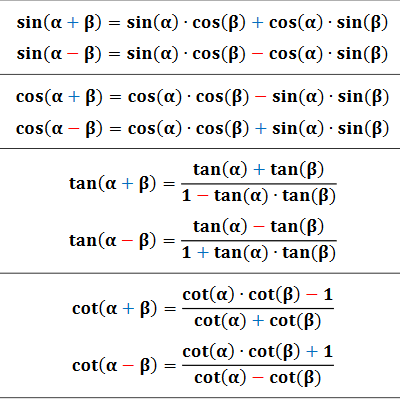
\includegraphics[scale=0.6]{trig/trig1.PNG}\\
\end{align*}
\textbf{Winkelfunktion des dreifachen winkel}
\begin{align*}
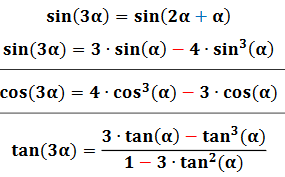
\includegraphics[scale=0.6]{trig/trig2.PNG}\\
\end{align*}
\newpage
\end{multicols}